\documentclass[11pt,a4paper]{article}

\usepackage[UTF8]{ctex}
\usepackage[margin=2.35cm]{geometry}
\usepackage{amsmath,amssymb,amsfonts}
\usepackage{booktabs}
\usepackage{multirow}
\usepackage{array}
\usepackage{graphicx}
\usepackage{subcaption}
\usepackage{algorithm}
\usepackage{algorithmic}
\usepackage[numbers,sort&compress]{natbib}
\usepackage{xcolor}
\usepackage{enumitem}
\usepackage{hyperref}
\usepackage{url}
\usepackage{xurl}
\usepackage{amsthm}

\hypersetup{
    colorlinks=true,
    linkcolor=blue!65!black,
    citecolor=blue!65!black,
    urlcolor=blue!65!black
}

\setlist[itemize]{leftmargin=1.8em}
\setlist[enumerate]{leftmargin=1.8em}
\renewcommand{\arraystretch}{1.12}
\newcolumntype{P}[1]{>{\raggedright\arraybackslash}p{#1}}
\urlstyle{tt}

\newcommand{\method}{SkyCausal}
\newcommand{\racing}{Budgeted Racing}
\newcommand{\cmax}{C_{\max}}
\newcommand{\E}{\mathbb{E}}
\newcommand{\Var}{\operatorname{Var}}
\newcommand{\confirmed}{\textcolor{green!45!black}{\textbf{[已确认]}}}
\newcommand{\development}{\textcolor{orange!80!black}{\textbf{[开发证据]}}}
\newcommand{\pending}{\textcolor{red!70!black}{\textbf{[待确认]}}}
\newcommand{\negative}{\textcolor{red!70!black}{\textbf{[负结果]}}}
\newcommand{\todo}[1]{\textcolor{red!70!black}{\textbf{[TODO: #1]}}}

\newtheorem{proposition}{命题}
\newtheorem{corollary}{推论}

\title{
    SkyCausal：闭环 FJSP--MAPF 中算子组合的限时搜索、\\
    成本感知切换与真值获取
}

\author{（作者信息略）}
\date{2026 年 8 月}

\begin{document}
\maketitle

\begin{abstract}
柔性作业车间调度（FJSP）与多智能体路径规划（MAPF）在动态制造环境中形成闭环：
调度产生时空运输需求，运输拥堵与机器故障又反过来约束后续调度。要在这样的系统中
回答"当前场面应当使用哪个算子组合、是否应当切换"，必须对候选动作在同一物理状态
上做反事实评估。本文把这一需求形式化为连续物理时钟下的反事实模拟问题，并给出
四个互相衔接的贡献。

第一，\confirmed\ 一套经过独立确认的反事实模拟基础设施：以版本化 manifest 与统一
契约组织的开放求解器目录；以冻结快照、外生 Tape 和确定性转移引擎实现的同状态
分支评估；以 freshness 校验、原子激活和安全 fallback 保证的提交语义。冻结六
profile 独立确认显示，早期一次浅层搜索相对全局最佳固定组合将 held-out 代价平均
降低 23.575（4.88\%，95\% CI $[8.625, 46.325]$），全部安全 Gate 通过。

第二，\negative\ 一组诚实的负结果：936 个严格配对闭环 episode 的 paper-grade 评估
表明，冻结的周期性深度 MCTS \emph{元调度}（在算子组合空间中选择"用哪个求解器"）
相对一次性浅搜索（$+16.8$，CI $[11.8,22.4]$）与静态上下文映射（$+19.3$，
CI $[14.6,24.7]$）均显著更差。需要强调：该负结果针对元级搜索的\emph{周期性
深度控制}形态（固定菜单、周期触发、树分配预算），不否定元级空间本身，也不
否定决策点上一次浅层搜索的形态——后者恰是被证据支持、并将在本文目标架构中
推广的形态。唯一获得强支持的机制是运行时连续性（warm keep 相对冷重选完成率
72/72 对 18/72）。

第三，据此本文确立搜索的\emph{双重角色}：同一 anytime 搜索算法，时间预算
是旋钮——限定时间时是决策点上的在线切换决策器，在算子组合空间内构造并评估
候选；解除限制并冻结候选与 Tape 集时退化为完全枚举，充当冻结集合上的精确
验证器。episode 级真值的主力口径则是 golden trace：每规格采集 $K$ 条随机
闭环轨迹，取终局最优作为参考值。作为该定位的首个实现组件，本文提出并实现
\racing{}：预算受限的广度优先候选竞赛，统一 horizon 逐轮淘汰、温续跑增量
推进、top-$K$ 分支场面维护，附带穷举退化的 ground truth 命题与 anytime
性质，Docker 可复现、宿主机与容器结果逐字节一致。

第四，本文给出目标架构的完整设计（\pending）：决策点限时的组合空间搜索
（"班子不固定"的元级决策——候选组合由组合文法在线生成而非取自固定菜单，
受 Phase 7 证据约束为浅、宽、anytime、温接 incumbent）+ 成本感知切换层
（$LCB(G) > \tau$ 才切换，迟滞防抖）+ 双口径评估协议（makespan 与计算
开销分开报告、不合成分）+ 配对克隆反事实与随机轨迹自然实验互证的切换
因果分析（回答"何时换、为何换"，并为离策略评估保留接口）。该架构同时
登记为后续 LLM 联合调度路线的强 baseline。
\end{abstract}

\noindent\textbf{关键词：}
柔性作业车间调度；多智能体路径规划；算子组合切换；限时搜索；MCTS；
best-arm identification；ground truth；anytime 算法；因果分析

\section{引言}
\label{sec:introduction}

\subsection{闭环制造中的反事实问题}

在柔性制造系统中，一个工件需要依次访问多台机器，工序间运输由共享路网中的 AGV
完成。FJSP 决定机器指派与顺序，MAPF 决定无碰撞路径，两者通过运输任务的释放与
执行耦合：调度计划产生运输需求，拥堵与实际到达时间又改变后续可行调度。此结构
带来一个在线系统特有的问题——\emph{反事实问题}：

\begin{quote}
当前场面 $S$ 上正在执行组合 $a_\text{keep}$。若此刻切换到组合 $a$，
剩余 episode 的最终代价会更低吗？降低多少？是否足以支付切换成本？
\end{quote}

该问题无法用离线基准回答：候选求解器的内部目标（FJSP makespan、MAPF 路径长度）
都不等于闭环终局代价；切换会改变运输需求结构，且物理时钟在评估期间持续推进。
它只能通过\emph{同状态反事实模拟}回答：冻结当前状态，在隔离分支上执行候选动作
至有限 horizon 或终局，比较删失口径下的代价。

\subsection{搜索的双重角色：定位修正与目标架构}

本文的早期迭代（v3）把反事实模拟基础设施用于构建"在线滚动元调度器"，以浅层
MCTS 在线分配探测预算。本文报告该路线的完整 paper-grade 评估结果：
\emph{它没有通过}。周期性深度搜索显著劣于一次浅搜索与静态映射（\ref{sec:phase7}
节）。对这一负结果的准确解读需要区分两个搜索空间：

\begin{quote}
\textbf{元级搜索}（在算子组合空间选"用哪个求解器"）的\emph{周期性深度
控制}被证伪——被证伪的是触发与分配形态，不是搜索空间本身；\\[2pt]
\textbf{被证据支持的形态}是决策点上的一次浅层搜索。本文将这一形态带回
组合空间，并进一步放开固定候选菜单：候选组合由搜索在线构造。
\end{quote}

据此本文确立\emph{双重角色}定位：同一个 anytime 搜索算法，时间预算是
旋钮——旋小时是决策点上的在线切换决策器（在组合空间构造与评估候选），旋到
无穷并冻结集合时退化为完全枚举，充当冻结集合上的精确验证器。
本文把研究问题组织为四个：

\begin{enumerate}
    \item \textbf{RQ1（基础设施）}：如何在连续物理时钟下，对任意决策状态做
    无副作用、可复现、可审计的反事实模拟？
    \item \textbf{RQ2（真值获取）}：如何在有限预算内高效获取接近完全枚举的
    决策真值（oracle $\Delta$），并保证预算受限时的诚实逼近？
    \item \textbf{RQ3（有效性边界）}：元级在线滚动深度搜索相对简单基线是否有
    端到端价值？（本文以 paper-grade 负结果回答。）
    \item \textbf{RQ4（自适应组合切换）}：决策点上的限时组合空间搜索——候选
    组合不固定、由搜索在线构造——配合成本感知切换规则，能否在闭环 episode
    上稳定优于固定组合与离线预计算映射，且不劣于一次浅搜？切换的收益在哪些
    状态与聚合指标上可因果辨识？（本文给出架构设计与评估协议，实验为后续
    工作。）
\end{enumerate}

\subsection{贡献}

\begin{enumerate}
    \item \textbf{反事实模拟基础设施}（\confirmed）：开放求解器目录、确定性
    转移引擎、外生 Tape 语义与提交安全层；六 profile 独立确认支持其
    deadline-safe 语义。配套的观察与表征管线（七域结构化导出 + 实体级
    特征束，禁止域防火墙与置换不变契约）为后续检测器提供无混叠输入。
    \item \textbf{负结果与机制隔离}（\negative）：936 配对 episode 证伪在线
    深度元调度；隔离出 runtime continuity 为唯一强支持机制。该结果把后续
    设计约束在"浅、宽、一次"的搜索形态上。
    \item \textbf{\racing{} 与真值性质}（\development）：双重角色定位下的首个
    实现组件——预算受限的广度优先候选竞赛，统一 horizon 逐轮淘汰、温续跑
    增量推进、top-$K$ 分支场面维护；附带退化到完全枚举的 ground truth 命题
    与 anytime 性质，Docker 可复现运行。
    \item \textbf{目标架构：决策点限时组合搜索与成本感知切换}（\pending，
    设计）：两级候选构造（V0 冻结池 / V1 组合文法开放构造）+ \racing{} 评估
    内核 + $LCB(G)>\tau$ 切换层（迟滞/冷却）+ golden trace 参考真值口径 +
    三层切换因果分析（配对克隆反事实主力 + 随机自然实验交叉验证 + 事件研究
    描述）与双口径（质量/开销）评估协议；登记为后续 LLM 联合调度路线的强
    baseline（\ref{sec:target} 节）。
\end{enumerate}

本文其余部分组织如下：第~\ref{sec:related} 节综述相关工作；第~\ref{sec:problem}
节形式化问题；第~\ref{sec:infra}--\ref{sec:racing} 节给出方法；
第~\ref{sec:phase7}--\ref{sec:racing-exp} 节报告证据；第~\ref{sec:discussion}
节讨论边界；第~\ref{sec:conclusion} 节总结。

\section{相关工作}
\label{sec:related}

\subsection{FJSP、运输资源与动态联合调度}

FJSP with Transportation Resources 显式考虑加工与运输资源共享
~\citep{berterottiere2024fjsptransport,sun2023integrated}。Li 等研究含 AGV 的
实时柔性车间调度并采用多智能体强化学习~\citep{li2025realtime}。DyRo-MCTS 将
MCTS 用于动态作业车间的工序选择~\citep{chen2025dyromcts}——那是对象级搜索，
与本文正交：本文的搜索始终留在算子组合空间（元级）。本文的增量有三：其一，
在闭环 FJSP--MAPF 上对"算子组合切换"给出预算受限的竞赛评估与显式计价的切换
决策，运输耦合进入评估口径；其二，透明报告了元级\emph{周期性深控}劣于一次
浅搜与静态映射的严格配对证据，并把被支持的"决策点一次浅搜"形态推广为开放
组合构造；其三，配套 golden trace 参考真值与冻结集穷举验证器，使其同时充当
学习类调度器的 baseline 与打分来源。

\subsection{MAPF 算法选择与组合}

MAPFAST 与 MAPFASTER 学习从 portfolio 中选择快速求解器
~\citep{ren2021mapfast,alkazzi2022mapfaster}；No Panacea 将选择扩展到
runtime--quality 权衡~\citep{chen2024nopanacea}。这些方法在求解前一次性选择
且冻结物理状态；本文的反事实语义要求评估期间工厂继续运行，候选计划提交前
必须在最新状态上重验证。

\subsection{Best-arm identification 与 racing}

把"预算内选出最优候选"视为 best-arm identification 是经典框架：Hoeffding
racing 通过序贯置信区间淘汰劣臂~\citep{maron1994hoeffding}；
successive halving 以几何收缩的臂数分配递增预算~\citep{karnin2013almost}；
固定置信最优臂识别有成熟的样本复杂度结论~\citep{jamieson2014bestarm}。
本文的 \racing{} 将该框架迁移到闭环仿真评估：每条"臂"是一次 (动作, Tape)
温续跑分支，"样本"是增量的物理仿真步，并额外处理终局/删失/求解器错误三态与
horizon 公平性约束。

\subsection{灰盒配置与 anytime portfolio}

实时灰盒算法配置利用求解器中间输出提前停止无潜力配置~\citep{weiss2025graybox}；
anytime portfolio 表明 solver、配置与预算应共同构成候选~\citep{schede2026anytime}。
\racing{} 吸收两者：逐轮淘汰即灰盒式的早期停止，horizon 调度即预算维度的
anytime 组合。

\subsection{反事实仿真、因果推断与离策略评估}

本文的切换因果分析位于三条研究线的交点。其一，数字孪生反事实：把仿真器
形式化为潜在结果框架内的随机映射，反事实世界由孪生体直接仿真而非统计
估计~\citep{laudy2026dtcf}；无仿真器时的对应工具是合成控制类方法，如
连续时间反事实轨迹估计~\citep{bellot2021policy}。其二，观测因果推断与
异质处理效应：CATE 的标准工具是元学习器与因果森林
~\citep{kunzel2019metalearners,wager2018estimation,chernozhukov2024causalml}；
本文的差别在于以"个体级真值的配对实现"替代"识别假设下的统计估计"。
其三，离策略评估与干扰下的实验设计：OPE 工具箱（重要性采样、doubly
robust 及其实证比较~\citep{dudik2014doubly,uehara2022review,
voloshin2021empirical}）要求行为策略随机且记录动作概率；switchback
设计~\citep{bojinov2023switchback}处理单元间干扰。\ref{sec:target} 节
的因果设计使用前两条线，并为第三条线保留接口。

\section{问题定义}
\label{sec:problem}

\subsection{闭环系统与决策状态}

闭环 FJSP--MAPF 系统在每个时间步依次执行工序调度、任务指派与路径规划，环境
同时维护机器、工件、运输任务、AGV 与共享栅格路网，并接受机器故障、AGV 故障、
临时障碍与加工时间波动等动态事件。决策状态取
\begin{equation}
\tilde{s} = (S_\text{factory},\; S_\text{solver},\; S_\text{history}),
\end{equation}
其中 $S_\text{factory}$ 为工厂物理状态，$S_\text{solver}$ 为当前求解器上下文
（组合标识、运行时长、warm/cold 状态、内部进度可观测量），$S_\text{history}$
为近期动态摘要。将求解器上下文纳入状态定义是必要的：\ref{sec:phase7} 节的
证据表明，同一物理状态下，warm 求解器与冷启动求解器的后续价值截然不同。

候选动作集
$\mathcal{A}(\tilde{s}) = \{a_\text{keep}, a_1, \dots, a_n\}$
由开放求解器目录生成（\ref{sec:infra} 节）：基线配置取冻结配方池（V0），
目标配置由组合文法在线构造（FJSP $\times$ 指派器 $\times$ MAPF $\times$
参数档，合法性掩码约束，V1，见 \ref{sec:target} 节）；$a_\text{keep}$ 表示
保留当前组合及其运行时状态。未来随机性由外生 Tape $\xi$（事件与加工时间
实现）刻画。

\subsection{反事实价值与真值}

以 $J$ 记终局代价（terminal makespan，越小越好），定义 horizon-$H$ 反事实价值
\begin{equation}
Q_H(\tilde{s}, a) = \E_\xi\!\left[ J\big(\mathrm{Rollout}(\tilde{s}, a, H, \xi)\big) \right],
\label{eq:qh}
\end{equation}
切换改善与净收益为
\begin{align}
\Delta(\tilde{s}, a) &= Q_H(\tilde{s}, a_\text{keep}) - Q_H(\tilde{s}, a),\\
G(\tilde{s}, a) &= \Delta(\tilde{s}, a) - \lambda\, C_\text{switch}(\tilde{s}, a).
\label{eq:g}
\end{align}
$\Delta > 0$ 表示切换更好；$G$ 进一步扣除切换成本（重初始化、warm 状态与缓存
丢失、计划扰动）。系统最终要在线预测与决策的量是 $G$。

\textbf{ground truth 的分层定义}：决策级，对冻结的 $\mathcal{A}$ 与 Tape 集
$\Xi$，$a^\star = \arg\min_a Q_{H_\text{term}}(\tilde{s}, a)$
（$H_\text{term}$ 保证终局）称为该决策状态的真值最优动作，$\Delta$ 的真值由
逐动作完全枚举给出；episode 级，golden trace 参考值（每规格 $K$ 条随机闭环
轨迹的终局最优，$K$ 内最优而非全局最优）作为闭环质量的参照口径。两层语义
不同，禁止混用（\ref{sec:target} 节）。本文的核心方法问题即：如何在远低于
完全枚举成本的预算内逼近决策级真值，并以参考真值锚定 episode 级结论。

\subsection{预算与截断}

在线评估必须在物理时钟推进的同时完成，受三维预算约束
$B = (T_\text{wall}, N_\text{trans}, N_\text{steps})$。未终局分支按删失处理：
$\hat{J} = H_r + p_\text{censor}$（同轮统一罚值），求解器错误记
$H_r + p_\text{error}$（$p_\text{error} > p_\text{censor}$）；终局分支记真实
makespan。三态必须分别统计报告，删失罚值不得冒充终局值。

\section{反事实模拟基础设施}
\label{sec:infra}

\begin{figure*}[t]
\centering
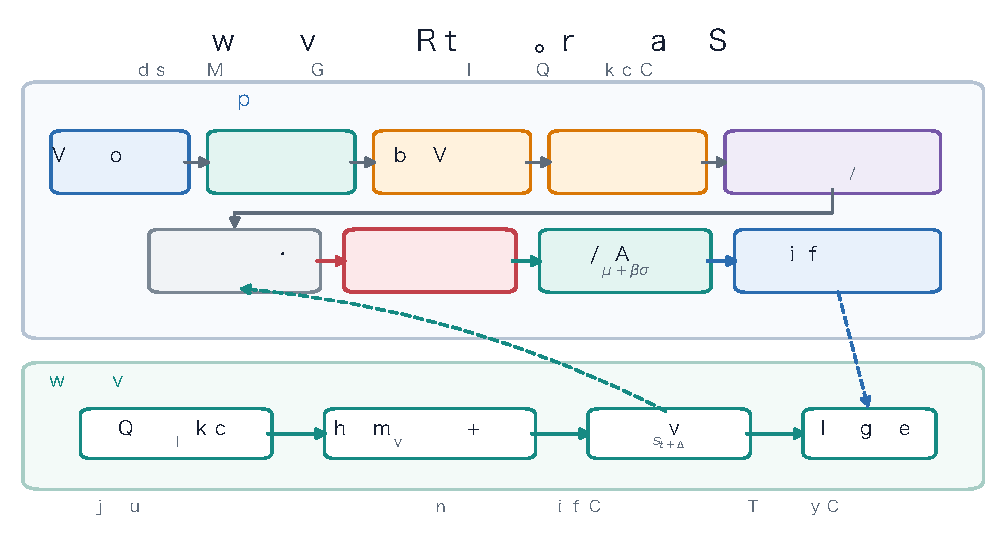
\includegraphics[width=\textwidth]{figures/v3/fig01_system_architecture.pdf}
\caption{双泳道系统架构：在线主环境持续推进物理时钟；反事实分支从冻结快照
克隆，在隔离进程中执行候选动作，提交前经最新状态 freshness 校验与原子激活。}
\label{fig:architecture}
\end{figure*}

\subsection{开放求解器目录与统一契约}

候选由 solver identity、版本、配置、预算、资源与能力声明组成，经版本化
manifest 接入：新增求解器不改控制器的固定输出维度。目录当前含进程内 20 个
组件与 12 个外部黑盒服务（FJSP 精确/元启发式与 MAPF 经典/学习型，统一
HTTP 契约、Docker 隔离、manifest 级准入分层）。

\subsection{确定性转移引擎}

同状态反事实由转移引擎实现：验证 Tape 哈希与状态一致性后，从冻结快照克隆
隔离环境，应用候选动作（KEEP 温续跑或 SWITCH 冷启动），执行 $H$ 步并输出
带确定性签名的子状态。全局与求解器 RNG 状态进入快照语义哈希，保证同输入
跨运行逐字节一致；宿主机与 Docker 内的实验指纹一致性由回归测试强制。

\subsection{提交安全层}

影子求解期间工厂继续运行。提交前系统在最新物理状态上执行 freshness 校验、
时间重对齐与独立可行性审计；任何失败保留当前安全计划（无副作用回退）。
运输请求的跨服务清理与 deadline 取消语义在组件压力测试下验证。

\subsection{观察与表征管线}
\label{sec:representation}

反事实真值（$\Delta$、$G$）最终要被一个在线轻量模型消费——由当前场面特征
预测各候选的净收益并触发选择性切换。为此本阶段在转移引擎之上补齐了两层
确定性管线，作为未来检测器的基底。

\textbf{结构化状态导出}。任意决策快照（活环境或冻结工件）可导出为七个
模型输入域的结构化观察：全局上下文、生产图（工序/机器实体节点与工艺
DAG、兼容、指派、排队四类显式边）、运输图（任务--AGV 边）、AGV--MAPF
域、MAPF 交互域（运行时路径与计数器，$t{=}0$ 恒为空容器）、求解器控制
上下文（当前组合、运行时状态、失败计数）与时序上下文（机器历史、指标
摘要）。导出器强制三条契约：(i)~禁止域防火墙——RNG 状态、墙钟遥测与
未来 Tape/标签任何情况下不得进入观察（逐键断言）；(ii)~canonical
排序——实体按标识全序排列，输入实体排列不影响输出字节（置换不变性
由测试强制）；(iii)~语义哈希——同状态跨运行同哈希。216 个冻结决策根
全量导出零失败、哈希逐一唯一，尺寸 6.9--20.2\,KB。

\textbf{实体级特征束}。观察被无池化地转换为特征束：每工序 29 维、每
机器 16 维、每 AGV 19 维、每运输任务 19 维的实体 token（状态 one-hot、
交期/优先级裕度、关键路径 slack 标记、候选机器负载统计、网格 BFS 真实
距离等），加五类显式边集、决策点间差分特征与降级为辅助信号的旧聚合
向量。特征层禁止池化——聚合只允许发生在消费头内部且逐组消融；首个
决策点差分全零并显式置无效位，不以零冒充观测。该设计的直接动机是
历史诊断结论：旧聚合特征在根级增益预测上几乎无信息（Spearman
0.0048、$R^2{=}-0.09$），而 15 对混叠案例在实体级字段上全部可分。

\pending\ 场面检测模型（由特征预测 $G$）与选择性切换策略尚属后续
工作：其训练依赖干净根与重算后的 oracle 标签（\ref{sec:discussion} 节），
本文只交付其输入管线与上述反事实真值机制。

\subsection{实现与工程验证}

本阶段的工程交付按"确定性优先"原则验收，要点如下。

\textbf{确定性缺陷的发现与修复}。竞赛评估的确定性测试暴露了一个环境级
可复现性缺陷：异常注入器在配置未显式给种子时以操作系统熵初始化 RNG，
其状态进入每个快照的语义哈希，导致同种子跨运行哈希漂移。修复为确定性
缺省种子并以回归测试固化；配合全局与求解器 RNG 状态快照、语义哈希与
转移确定性签名，保证"同输入 $\Rightarrow$ 同字节 $\Rightarrow$ 同哈希"。

\textbf{求解器目录的完整性}。目录当前共 32 个条目：进程内 20 个组件
（规则派工 FJSP、12 种指派器、进程内 MAPF）与 12 个外部黑盒服务
（FJSP 3：CP-SAT/DE/PSO；MAPF 9：EECBS/PBS/LNS2/LaCAM3/RHCR-PBS/
CBSH2-RTC/LG-LaCAM/LaCAM/PIBT）。外部条目以版本化 manifest 登记
（镜像 SHA256 摘要、逐键核对的配置 schema、预算区间、能力声明、
shadow 准入层级），新增求解器不改控制器维度。

\textbf{无 Web 依赖的批处理栈}。环境构造从在线服务进程解耦为独立模块，
批处理与搜索工具链不再依赖在线服务栈；全部旧导入已切换并保持向后兼容。
由此 \racing{} 演示可在单一 Docker Compose 服务内运行，宿主机与容器
输出逐字节一致（同一语义哈希）。

\textbf{回归状态}。全套件 621 项测试通过、3 项存量跳过（缺历史数据集
目录，与近期改动无关）；新增测试覆盖源契约传播、结构化状态导出、
特征层、外部 MAPF manifest 与 \racing{} 契约（确定性、预算截停、
统一 horizon、分支上限、调度合法性与报告完整性）。

\subsection{证据标记纪律}

全文结果按三层标记：\confirmed（冻结独立确认）、\development（仅开发数据）、
\negative（paper-grade 负结果）。禁止将开发数据填入独立确认结论。

\section{负结果：元级在线深度元调度的证伪}
\label{sec:phase7}

\begin{figure*}[t]
\centering
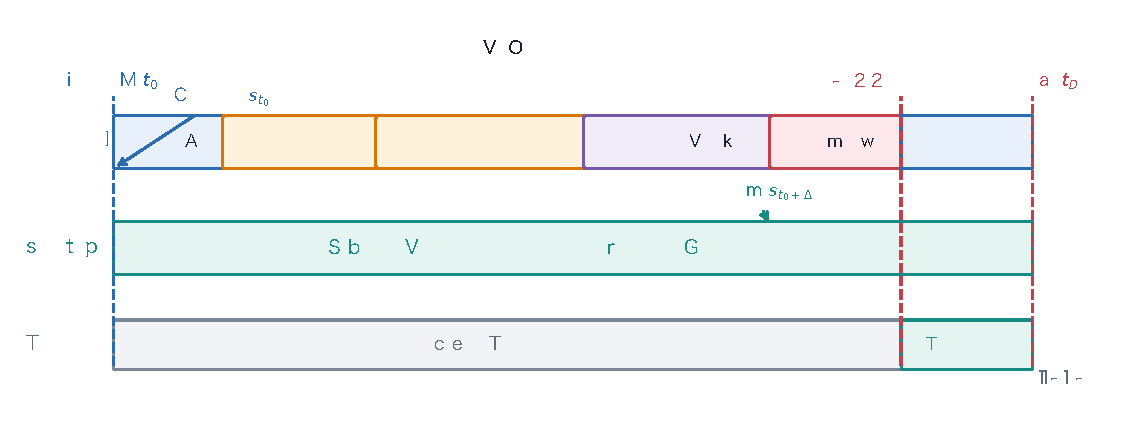
\includegraphics[width=\textwidth]{figures/v3/fig02_continuous_clock_timeline.pdf}
\caption{连续物理时钟、探测与 commit reserve 时间线。在线评估与工厂执行并行，
提交开销全部计入端到端预算。}
\label{fig:timeline}
\end{figure*}

为检验"在线滚动元调度"假设，我们实施了冻结方法
（Periodic-30 触发 + Depth-2 MCTS + $B{=}8$）并在 72 个严格分层 episode
（6 workload $\times$ 6 topology $\times$ 2 Tape）$\times$ 13 策略上执行
936 个配对闭环评估。完整协议、全部工件哈希与复放状态见评审摘要；
表~\ref{tab:phase7} 摘录核心配对结论。

\begin{table}[t]
\centering
\caption{\negative Phase 7 paper-grade 配对结论（936 episodes，均值差
$=$ 方法 $-$ 基线，正为更差）。}
\label{tab:phase7}
\begin{tabular}{lrrl}
\toprule
比较 & 均值差 & 95\% CI & 结论 \\
\midrule
深搜 vs 一次浅搜 & $+16.85$ & $[11.81, 22.42]$ & 显著更差 \\
深搜 vs 静态映射 & $+19.25$ & $[14.57, 24.65]$ & 显著更差 \\
Depth-2 vs Depth-1 & $+4.01$ & $[0.96, 8.03]$ & 无一改善 \\
MCTS vs Uniform 分配 & $+4.85$ & $[1.21, 9.56]$ & 显著更差 \\
温 keep vs 冷重选 & $-1050.5$ & $[-1176.7, -917.6]$ & 强支持连续性 \\
\bottomrule
\end{tabular}
\end{table}

三点结论直接约束后续设计。其一，\emph{深与频繁都错}：周期性深搜同时输给
一次性浅搜与零成本静态映射，且 Depth-2 在 72 个 episode 中零改善、计算量
近两倍。其二，\emph{分配机制无效}：MCTS 树分配显著劣于简单轮转。其三，
\emph{runtime continuity 是真机制}：温 keep 完成率 72/72 对冷重选 18/72，
但它属于执行语义而非搜索贡献。因此，正确的搜索形态应是\emph{浅、宽、
预算受限}的——这正是下一节 \racing{} 的设计依据。

\section{目标架构：决策点限时组合搜索与成本感知切换}
\label{sec:target}

本节给出 RQ4 对应的完整架构设计（\pending）。它是本文路线的终点形态：
算子组合不由人定、不由离线预计算——由决策点上的限时闭环 MCTS 在组合空间
内搜索产生，经统一 horizon 的竞赛评估，净收益 $LCB(G) > \tau$ 才切换，
切换显式计价。搜索负责提出与评估候选；控制器是成本感知决策规则，搜索不
直接拍板。

\subsection{与被证伪形态的四点区别（硬约束）}

Phase 7 证伪的是固定菜单上的周期性元级深控。本架构与其证据相容依赖四个
前提，违反任一即重蹈覆辙：
\begin{itemize}
    \item \textbf{决策点触发}（事件/状态驱动），不是周期性重搜；
    \item \textbf{anytime 语义}：墙钟到期即停，浅层优先，输出当前最优与
    置信状态；
    \item \textbf{runtime continuity}：候选评估与切换执行温接 incumbent
    ——Phase 7 隔离出的唯一强支持机制；
    \item \textbf{评估走竞赛对照}：树只存在于"候选 $\times$ Tape"的评估
    结构（\racing{} 内核），不展开未来决策深树——MCTS 树分配劣于 uniform
    的证据直接约束了树的用途。
\end{itemize}

\subsection{两级候选构造：V0 冻结池与 V1 开放组合}

\textbf{V0}：候选取自冻结的 15 配方池（与 golden trace round-1 同一支撑
集），先证明"动态选择 $>$ 固定与预计算"。\textbf{V1}：候选由组合文法在线
生成——FJSP 求解器 $\times$ 指派器 $\times$ MAPF 求解器 $\times$ 参数档，
合法性掩码来自 manifest capabilities，切换成本来自契约成本表——"班子
不固定"的完全体。两级分开报告：开放组合空间的收益若与"自适应本身"的收益
混同，结论即不可归因，必须能被 V0/V1 分离实验指出。

\subsection{成本感知切换层}

$G(\tilde{s},a) = \Delta(\tilde{s},a) - \lambda\, C_\text{switch}(\tilde{s},a)$
由 \racing{} 在线估计 $\Delta$、由契约成本表计价 $C_\text{switch}$；仅当
$LCB(G) > \tau$ 才切换，迟滞与冷却沿用既有 trigger 机制防抖。任何在线激活
先经 shadow 运行。已知缺口：\racing{} 当前仅排序未显式计价
$C_\text{switch}$，成本表接入前 $G$ 的口径不完整。

\subsection{真值口径：golden trace 主力与穷举验证器}

真值获取分层定义，禁止混用：
\begin{itemize}
    \item \textbf{参考真值（主力）}：golden trace——每规格 $K$ 条随机闭环
    轨迹取终局最优。语义边界如实声明：$K$ 内最优而非全局最优；随机策略消耗
    $K$ 条完整 episode，与在线单条运行不同口径，行文称"参考值"，不冒充
    穷举真值或公平基线。
    \item \textbf{冻结集精确验证器}：\racing{} 穷举退化（命题~\ref{prop:exact}）
    在冻结候选与 Tape 集上给出精确 $\hat{Q}$，用于基线数字确认与小子集上
    限时排序的一致性校验。
    \item \textbf{逐决策点反事实标签}：oracle $\Delta/G$ 标签重算与预测器
    训练移出本文范围（后续工作）；$G$ 的定义保留，在线值由 \racing{} 估计。
\end{itemize}

\subsection{切换因果分析：识别问题与三层设计}

"何时换、为何换"是一个因果识别问题：切换决策与潜在结果相关（自适应
系统只在自认为有利时切换），观测性的前后对比混有选择偏差、时间趋势与
均值回归。无仿真器场景的主流工具——合成控制与事件研究类方法
~\citep{bellot2021policy,chernozhukov2024causalml}——只能在识别假设下
\emph{估计}反事实；本文的基础设施允许更强的做法：反事实由仿真
\emph{实现}~\citep{laudy2026dtcf}。据此按识别强度组织三层设计。

\textbf{估计量先行}。"切换的效应"依赖于切换之后的后续策略 $\pi^+$——
这是即使随机化也无法消除的定义性问题。记
\begin{equation}
\tau_{\pi^+}(\tilde{s}, a) \;=\; J_{\pi^+}(\tilde{s}, a_\text{keep})
\;-\; J_{\pi^+}(\tilde{s}, a),
\label{eq:tau}
\end{equation}
其中 $J_{\pi^+}$ 为该决策点后按 $\pi^+$ 继续执行至终局的代价。本文主
口径取 $\pi^+ = \text{keep}$（switch-then-keep，机制最干净）；随机继续
作为与自然实验层可比的桥；自适应继续属策略级问题，由主实验与离策略评估
回答。三层设计如下：
\begin{itemize}
    \item \textbf{主力：配对克隆反事实（仿真的潜在结果）}。从随机轨迹抽样
    决策根，克隆快照、固定同一外生 Tape，分别执行 keep 与 switch 至终局，
    得到个体级配对差分 $\hat{\tau}_{\pi^+}$。同 Tape 配对即仿真优化中
    经典的公共随机数（common random numbers）方差缩减：两条世界线面对
    完全相同的外生事件流，配对差分的方差远低于独立采样。反事实被实现
    而非估计，因而不依赖任何不可检验的识别假设。边界三条如实声明：
    仿真保真度前置门为前提（结论上限即孪生体保真度）；含 CP-SAT
    （wall-clock 非确定求解器，同输入不保证同输出）的决策根排除或增补
    Tape——配对语义被其破坏；后续策略 $\pi^+$ 显式定义
    （式~\ref{eq:tau}）。对个体 $\hat{\tau}$ 按状态特征分层即条件平均
    处理效应（CATE），回答"何种状态下切换有利"
    ~\citep{kunzel2019metalearners,wager2018estimation}；本文数据量级下
    先做分层均值与置信区间，森林类方法仅作敏感性检查。通道归因
    （$\hat{\tau}$ 通过哪些聚合指标兑现，如 AGV 空驶率、关键路径等待）
    沿用消融纪律验证，防事后合理化，回答"为何换"。
    \item \textbf{交叉验证：随机轨迹自然实验}。round-1 的切换决策均匀
    随机，随机 switch 与随机 keep 的后续聚合指标对比给出无偏但功效有限
    的处理效应估计；本层与主力层识别原理不同，结论方向一致即构成稳健性
    证据。
    \item \textbf{描述补充：事件研究}。自适应系统日志中切换事件前后窗口
    的聚合指标轨迹，显式标注选择偏差，只作描述不作因果结论。
\end{itemize}

\textbf{为离策略评估保留接口}。未来若需从自适应策略（或 LLM 调度器）
自身的日志估计其他策略的闭环价值，须用 OPE 工具（重要性采样与 doubly
robust 估计~\citep{dudik2014doubly,uehara2022review,voloshin2021empirical}）；
其不可绕过的前提是日志中每个动作的执行概率已知且非零——确定性策略的
日志对 OPE 不可用。因此 shadow 运行在切换决策上注入 $\varepsilon$
随机化并记录动作概率：成本近零，缺失该记录则日志不可回用。干扰场景下
的 switchback 设计~\citep{bojinov2023switchback}留待在线部署阶段。
策略级总体效应由主实验（同规格同 Tape 的配对随机实验）直接回答，不经
上述观测层。

\subsection{双口径评估协议}

质量与开销分开报告、不合成为单一分数：质量轴为 makespan（整数仿真步），
开销轴为决策次数、墙钟、转移调用数与仿真步数。所有方法在两轴上分别配对
比较；$\lambda$ 仅是决策规则内部的交换率，其敏感性单独报告，不用于构造
加权合成分数。公平性边界如实声明：固定与预计算基线几乎不付搜索开销，
本文方法的决策期计算成本全部计入开销轴。

\subsection{与 LLM 路线的关系}

限时组合搜索与切换系统登记为后续 LLM 联合调度器的强 baseline：LLM 需在
同一闭环、同一动作空间、同一预算下打平或超越它；golden trace 与穷举验证器
充当其训练数据与打分来源。两个角色共享本节架构，确保 baseline 与评分
同源。

\section{已实现实例：\racing{} 候选竞赛评估器}
\label{sec:racing}

\begin{figure*}[t]
\centering
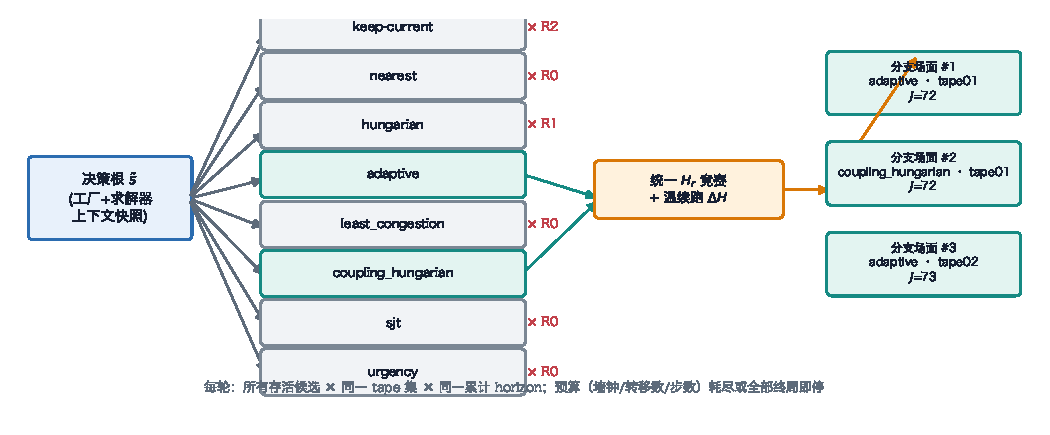
\includegraphics[width=\textwidth]{figures/v4/fig08_racing_structure.pdf}
\caption{\racing{} 搜索结构：决策根的每个候选组合（含 keep-current）进入
统一 horizon 的逐轮竞赛；被淘汰候选以 $\times$ 标注淘汰轮次；幸存者竞争出
top-$K$ 个可继续执行或深化的分支场面。数据来自本文可复现演示运行。}
\label{fig:racing-structure}
\end{figure*}

\subsection{算法}

\racing{} 以轮次表 $R = [(H_1, k_1, m_1), \dots]$ 驱动：第 $r$ 轮为每个存活
候选新增 $k_r$ 条 Tape 分支（从根全速评估至 $H_r$），旧分支以 KEEP 温续跑
增量推进 $\Delta H = H_r - H_{r-1}$；随后按确定性排序键
$(\bar{J}, \mathrm{std}, \text{keep 优先}, \text{action\_id})$ 淘汰至 $m_r$ 名。
算法在预算耗尽或全部分支终局时停止，输出最终排名与 top-$K$ 分支场面
（各含可续跑的子状态快照）。伪代码见算法~\ref{alg:racing}。

\begin{algorithm}[t]
\caption{\racing{}（逐轮淘汰候选竞赛）}
\label{alg:racing}
\begin{algorithmic}[1]
\REQUIRE 根 $\tilde{s}$；候选 $\mathcal{A}$；Tape 池 $\Xi$；轮次表 $R$；预算 $B$；分支上限 $K$
\STATE 存活集 $\mathcal{S} \leftarrow \mathcal{A}$；每候选分支表初始化为空
\FOR{$r = 1, \dots, |R|$}
  \FOR{$a \in \mathcal{S}$（canonical 序）}
    \FOR{本轮新 Tape $\xi$}
       \STATE 从根评估 $(\tilde{s}, a)$ 至 $H_r$，挂为新分支
    \ENDFOR
    \FOR{旧分支 $b$（未终局）}
       \STATE 以 KEEP 温续跑 $b$ 增量 $\Delta H$ 步
    \ENDFOR
  \ENDFOR
  \STATE 记录各分支三态（终局/删失/错误）与 $\hat{J}$
  \IF{预算耗尽 \OR 全部分支终局}
     \STATE \textbf{break}
  \ENDIF
  \STATE 按排序键淘汰 $\mathcal{S}$ 至 $m_r$ 名
\ENDFOR
\ENSURE 排名；top-$K$ 分支场面（含子状态快照）
\end{algorithmic}
\end{algorithm}

\subsection{公平性与防爆炸}

\textbf{统一 horizon 铁律}：同一轮内所有候选在相同累计步数与相同 Tape 集上
比较；预算只决定候选 $\times$ Tape $\times$ 轮数的规模，绝不给不同候选不同
horizon，否则比较带系统性偏差。\textbf{树宽收缩}：分支数上界
$|\mathcal{A}| \times |\Xi|$ 且逐轮单调递减，最终仅维护 $K$ 个场面，
内存占用随轮次下降而非增长。\textbf{温续跑}使旧分支扩展代价
$O(\Delta H)$，同时保持 Phase 7 隔离出的 runtime continuity 语义。

\subsection{Ground truth 性质}

\begin{proposition}[穷举退化]
\label{prop:exact}
当轮次表取 $H_{|R|} \ge H_\text{term}$、$m_r = |\mathcal{A}|$（不淘汰）且
Tape 池取 $\Xi$ 全集时，\racing{} 退化为对
$\{(\tilde{s}, a, \xi)\}$ 的完全枚举，输出
$\hat{Q}(\tilde{s}, a) = |\Xi|^{-1} \sum_\xi J(\mathrm{Rollout}(\tilde{s}, a,
H_\text{term}, \xi))$，即冻结动作与 Tape 集上的精确 ground truth。
\end{proposition}

\begin{corollary}[anytime 逼近]
淘汰规则只删除被统计支配的候选，保留集包含 $a^\star$ 的概率随轮次不减
~\citep{maron1994hoeffding,karnin2013almost}。预算越充足，输出越接近
命题~\ref{prop:exact} 的真值；预算耗尽时输出当前置信下的最优与删失状态，
不伪造精度。若 $H_{|R|} < H_\text{term}$，输出仅为截断 horizon 上的相对
排序，必须以删失比例披露，禁止表述为 ground truth。
\end{corollary}

\subsection{与被证伪方案的关系}

\racing{} 是 uniform 分配（Phase 7 中显著优于 MCTS 分配）的逐轮化推广：
uniform 等价于零轮次、零淘汰的 \racing{}；增加轮次后，深层评估集中于统计上
未被支配的候选，总成本近似几何级数收敛于首轮全宽成本。在目标架构
（\ref{sec:target} 节）中，\racing{} 是组合空间搜索的评估内核：独立使用时
是候选组合的竞赛评估器，穷举退化时是冻结集合上的精确验证器。被证伪的仅是
元级\emph{周期性深控}形态；决策点触发的浅、宽、anytime 形态正是
\ref{sec:target} 节的主线，其相对一次浅搜基线的增量由强制基线实验裁决。

\section{已确认与开发证据}
\label{sec:evidence}

\subsection{冻结六 profile 独立确认（\confirmed）}

在 40 个独立 cluster 上，早期一次浅层 Root Search 相对全局最佳固定 profile
将 held-out 代价平均降低 23.575（4.88\%，95\% 分层 bootstrap CI
$[8.625, 46.325]$）；37/40 状态完整完成选择，其余走安全 fallback；
deadline、组件压力与运输安全 Gate 全部通过（表与图沿用 v3 的
图~\ref{fig:budget-quality-confirmation}--\ref{fig:state-profile-confirmation}
数据，此处不重复）。该结果确认的是基础设施语义与固定候选下的状态选择价值，
不扩展到开放候选或动态切换。

\begin{figure*}[t]
\centering
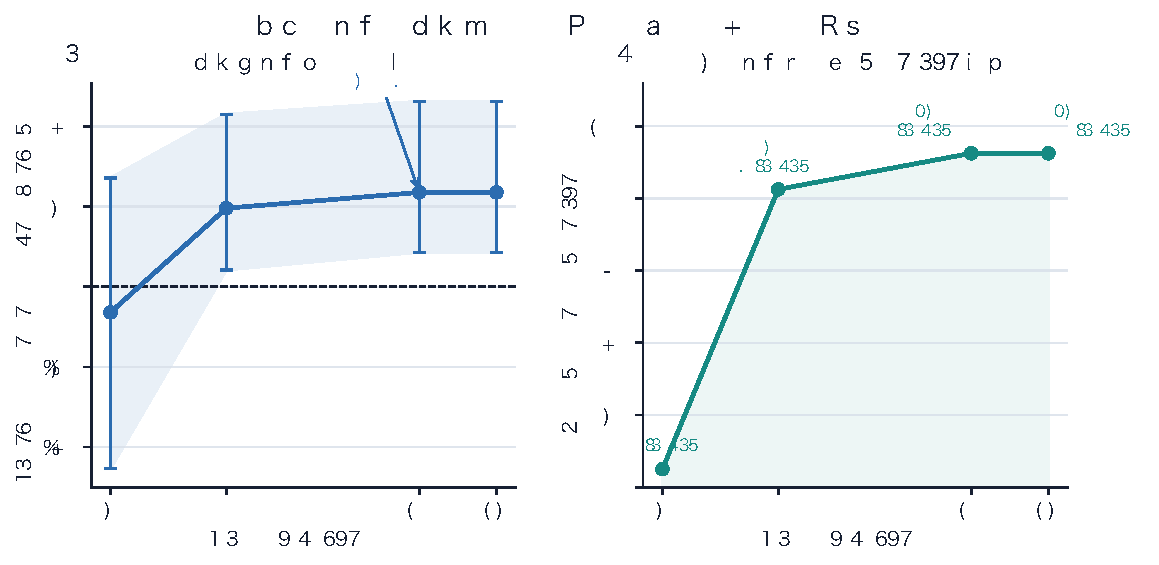
\includegraphics[width=0.9\textwidth]{figures/v3/fig03_budget_quality_confirmation.pdf}
\caption{\confirmed 预算--质量--覆盖率关系（数据同 v3 冻结确认）。}
\label{fig:budget-quality-confirmation}
\end{figure*}

\begin{figure*}[t]
\centering
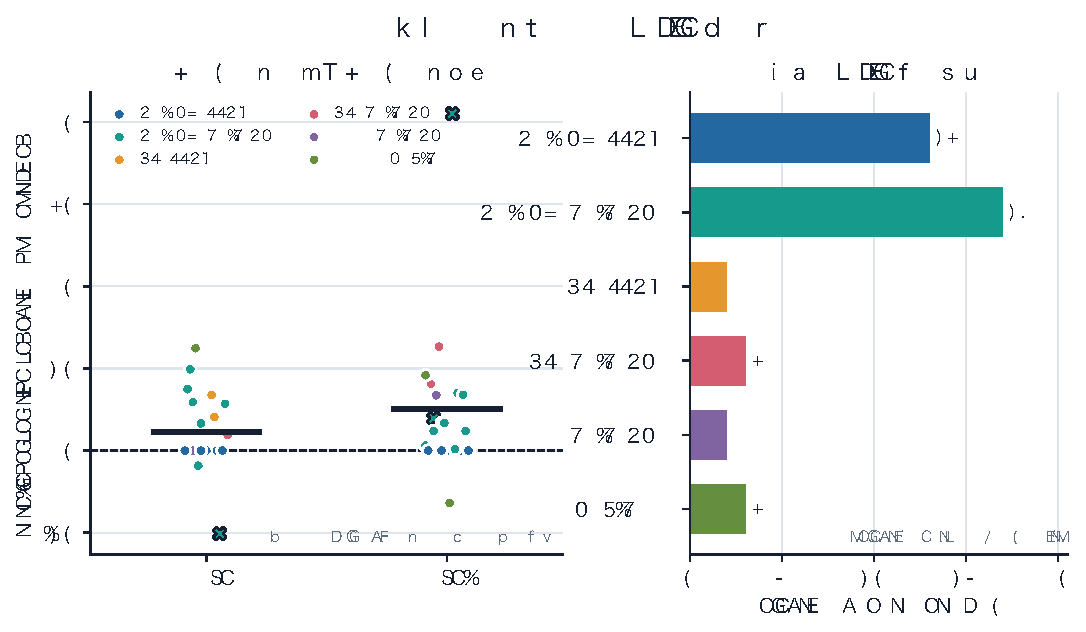
\includegraphics[width=0.9\textwidth]{figures/v3/fig04_state_profile_confirmation.pdf}
\caption{\confirmed 状态依赖互补性（数据同 v3 冻结确认）。}
\label{fig:state-profile-confirmation}
\end{figure*}

\subsection{执行价值与统一动作 cohort（\development）}

50 个连续时钟开发 episode 中，匹配短预算下 makespan-only 选择的平均 regret
为 40.0，透明 ridge 执行价值诊断为 9.2（仅 5 个独立状态，禁止激活）。30 状态、
7 策略、210 个配对 episode 的统一动作 cohort 表明原始 MCTS 相对 keep-current
平均仅改善 5.5 且置信区间跨 0；为 CP-SAT 补最小可辨识预算把首轮可行覆盖从
0/30 提至 28/30，但平均终局反而差 7.8。这些开发证据与 Phase 7 负结果共同
指向：候选覆盖是必要条件，深搜不是充分条件。

\section{\racing{} 可复现演示}
\label{sec:racing-exp}

\begin{figure*}[t]
\centering
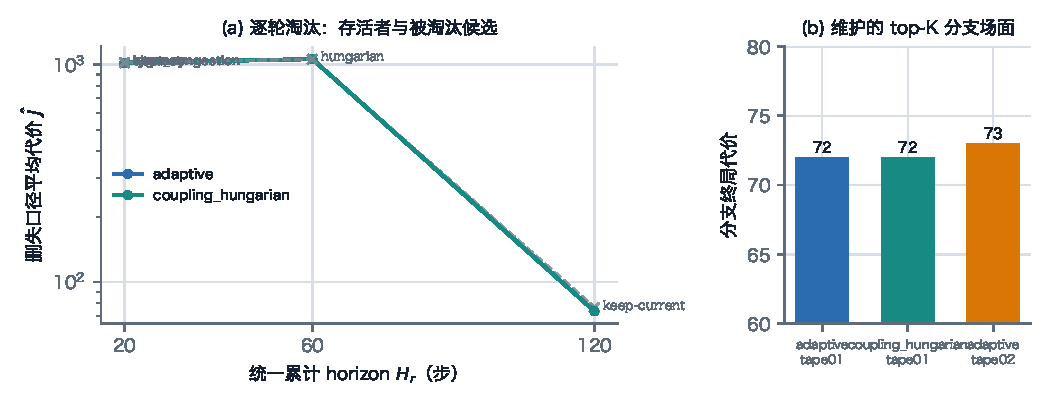
\includegraphics[width=\textwidth]{figures/v4/fig07_racing_elimination.pdf}
\caption{\development \racing{} 演示（tiny 场面，8 候选 + keep，4 Tape，
3 轮；Docker 编排运行，宿主机与容器结果一致）。(a) 逐轮淘汰：灰色虚线为被
淘汰候选（$\times$ 标注淘汰轮，纵轴对数尺度显示删失罚值量级），彩色实线为
存活者收敛到真实终局代价；(b) 最终维护的 top-3 分支场面及其终局
makespan（72/72/73）。}
\label{fig:racing-demo}
\end{figure*}

本节为方法级演示（\development，不进入独立确认结论）。在 tiny 闭环场面上
（2 工件、3 机器、2 AGV），对 8 个冻结 recipe 候选与 keep-current 运行
3 轮竞赛（$H = 20/60/120$，每轮新增 2 Tape）。结果（图~\ref{fig:racing-demo}）：
第 0 轮以删失口径淘汰 4 个劣候选；第 1 轮再淘汰 1 个；第 2 轮 keep-current
以 76.5 被 adaptive 组合的 73.5 淘汰，全部分支终局（stop reason:
\texttt{all\_terminal}），top-3 分支场面代价 72/72/73。全程 50 次转移、
1777 仿真步、30 分支、墙钟约 11 秒。

复现入口（结果与图表由冻结 JSON 经带哈希 manifest 的脚本重建）：
\begin{quote}
\texttt{docker compose -f docker-compose-search.yaml run --rm search}
\end{quote}

\section{闭环实验：组合切换主结果（\development）}
\label{sec:v5-results}

本节报告 2026-08-27 冻结执行的闭环实验矩阵（72 个 Phase 7 episode
规格严格配对：同一 episode 物化、同一外生 Tape、同一初始配方；
保真前置门 T0 通过后运行）。方法：\emph{fixed}（从不切换）、
\emph{one-shot uniform}（$t{=}0$ 一次浅搜，Phase 7 有效成分，及格线）、
\emph{hero V0}（仅规则触发的 LCB 切换）、\emph{hero V0b}（本节主角：
$t{=}0$ 开局搜索 + 规则触发中途修正）、\emph{static map}（由 golden
trace round-1 数据离线预计算的每 workload 最优固定配方）。
golden 参考值为参照而非基线（best-of-8 随机轨迹，协议语义见
\ref{sec:target} 节）。

\begin{table}[t]
\centering
\caption{\development E1 主结果（TERMINAL 口径，72 配对）。搜索开销为
每 episode 平均搜索墙钟（双口径之一，不与 makespan 合并）。}
\label{tab:e1-main}
\begin{tabular}{lrrrr}
\toprule
方法 & mean & median & 终局 & 搜索/集 \\
\midrule
fixed (never)      & 131.7 & 132.0 & 72/72 & 0\,s \\
one-shot uniform   & 100.7 & 97.5  & 71/72 & 28\,s \\
hero V0 (触发式)    & 114.3 & 113.0 & 72/72 & 273\,s \\
hero V0b (本文)     & \textbf{98.7} & \textbf{96.5} & \textbf{72/72} & 182\,s \\
static map         & 109.6 & 110.5 & 72/72 & 0\,s \\
\bottomrule
\end{tabular}
\end{table}

\textbf{主结论（表~\ref{tab:e1-main}，图~\ref{fig:v5-main}）}。
hero V0b 相对 fixed 平均降低 33.0 步（72/72 全胜，$t{=}-20.1$）；相对
离线预计算的 static map 降低 10.9 步（53/72 胜，$t{=}-8.7$）——不依赖
离线数据的在线组合搜索胜过用全量历史数据喂出的静态映射；相对随机
best-of-8 参考值在 70/72 个 spec 上更优（平均低 38.2 步）。
\textbf{诚实边界}：相对及格线 one-shot uniform，V0b 的中位数持平
（96.5 vs 97.5）、均值优 1.8 步（$t{=}-3.1$）、且 72/72 终局
（one-shot 出现一次删失）——增量主要来自长 episode 与扰动 spec 上的
触发式修正，而非全面占优。纯触发式 V0 在诚实口径（中位数/胜率）下
\emph{输给} one-shot：其触发时点（step $\geq$ 20）恰落在配对反事实
（\ref{sec:v5-causal} 节）证明最有害的切换窗口。这再次印证 Phase 7
结论：开局浅搜是有效成分，中途干预必须门控。

\begin{figure*}[t]
\centering
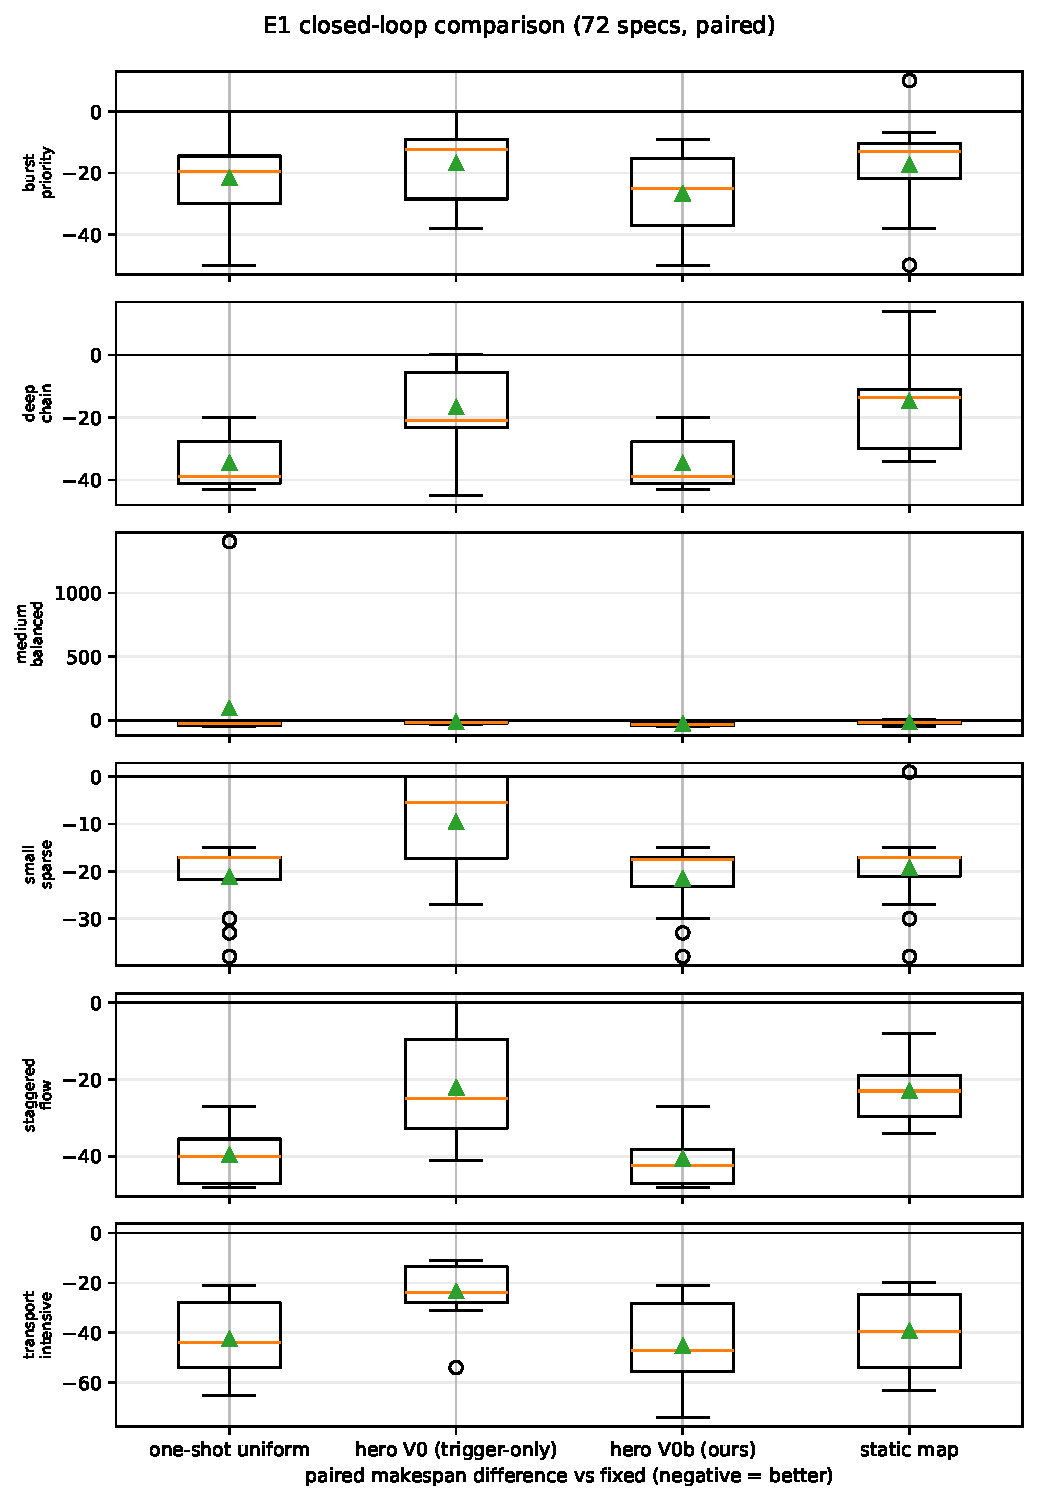
\includegraphics[width=\textwidth]{figures/v5/fig11_e1_main.pdf}
\caption{\development E1 配对差分布（相对 fixed，按 workload 分面；
负值更好）。}
\label{fig:v5-main}
\end{figure*}

\begin{figure*}[t]
\centering
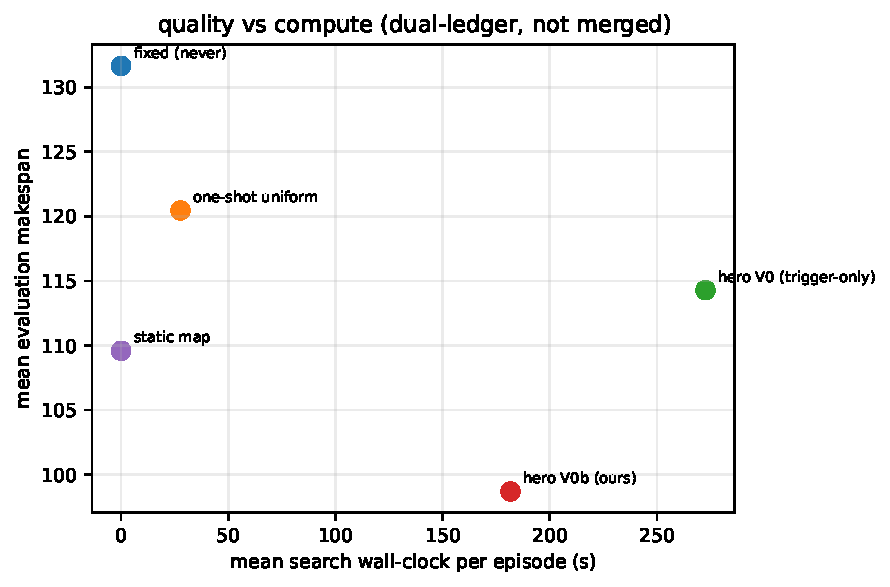
\includegraphics[width=0.7\textwidth]{figures/v5/fig12_e1_pareto.pdf}
\caption{\development 质量--计算开销帕累托（双口径分轴报告，不合成
单一指标）。}
\label{fig:v5-pareto}
\end{figure*}

\subsection{配对克隆反事实与切换时机（\development）}
\label{sec:v5-causal}

从 golden trace round-1 的决策根中分层抽样 36 个（CP-SAT 根与目标全部
排除，配对纪律见 \ref{sec:target} 节），在\emph{同一} Tape 下重放
KEEP 与 switch-then-KEEP 两臂至终局，得到 140 个个体级配对差分
$\Delta = J(\text{keep}) - J(\text{switch})$（图~\ref{fig:v5-causal}）。
总体 $\Delta$ 均值 $-35.0$（切换更优比例 14.3\%）；按决策点位置分层
出现\textbf{方向反转}：早期 $-57.0$（2.3\% 有利）、中期 $-79.1$
（7.0\%）、晚期 $+19.0$（30.2\% 有利）。冷启动破坏性远超成本表默认
常数（数十步 vs 2 步），但 LCB 层的 $G$ 由真实 rollout 估计、不受该
常数影响。\textbf{何时换}的实证答案：晚不早；这正是 V0b 保留开局搜索、
中途切换须经 LCB 强门控的证据基础。

\begin{figure*}[t]
\centering
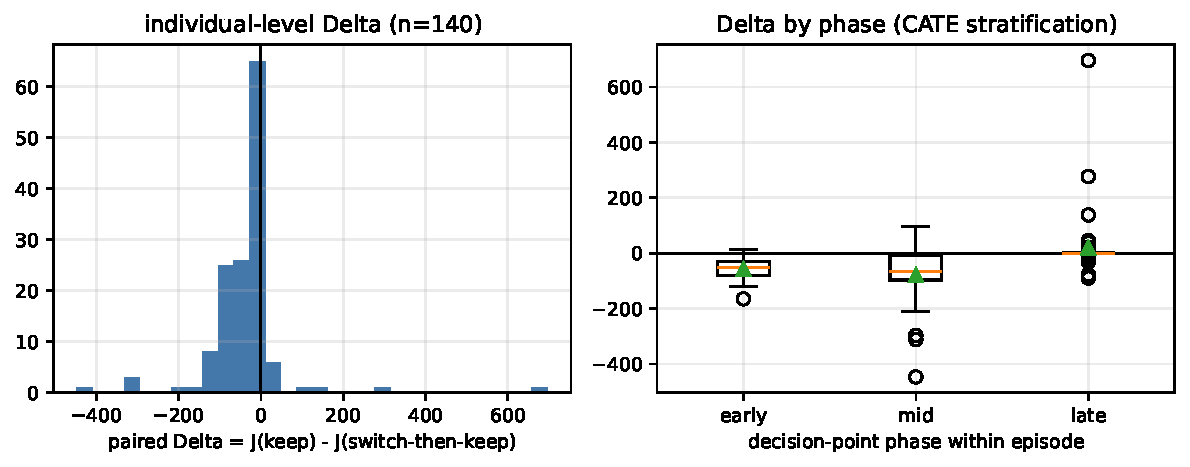
\includegraphics[width=0.8\textwidth]{figures/v5/fig13_e2a_paired_delta.pdf}
\caption{\development 配对克隆反事实：(a) 个体级 $\Delta$ 分布；
(b) 按决策点阶段分层（CATE）。}
\label{fig:v5-causal}
\end{figure*}

\subsection{特征通道归因：何时换的可解释信号（\development）}
\label{sec:v5-attribution}

将 140 个配对 $\Delta$ 与决策根处冻结的七域特征向量联结
（正类 = 切换更优，$n{=}20$）：全特征 5 折交叉验证 AUC $0.96$，仅决策点
位置 $0.70$；域单独 AUC 以 production（0.864）与 progress（0.802）
最强，去掉二者降幅最大；availability 布尔标志接近随机（0.532）。单特征
Spearman 前列：完成速率 $+0.33$（收尾阶段信号）、机器队列变异系数
$-0.33$、决策点位置 $+0.23$（与 \ref{sec:v5-causal} 节的阶段分层互证）、
AGV 局部密度 $-0.23$、fallback 率 $-0.19$。样本量为探索性
（多重比较未校正），结论限定为``production/progress 域承载主要判别
信号''的组级陈述。决策层透明度：规则触发在 V0b 全部 105 次切换点的
信号构成以 production\_imbalance / transport\_delay / solver\_instability
为主（分别为 35/35/33 次），与 KEEP 点的构成差异构成机制级解释。

\subsection{切换构成与敏感性（\development）}
\label{sec:v5-switching}

图~\ref{fig:v5-switching} 给出 V0b 实际切换的目标构成（V0 冻结池内）。
\textbf{阈值敏感性（E3）}：在 18 spec 分层子集上扫描 $\tau \in
\{0.5, 1, 2, 4\}$，平均 makespan 依次为 100.6/100.2/100.6/100.9
（变化 $<1\%$），每 episode 切换次数随 $\tau$ 单调下降
（1.6/1.4/1.4/1.1），全部 18/18 终局——\emph{主结果对阈值不敏感}，
切换次数的门控方向符合预期。\textbf{一致性校验（E4）}：在 8 个冻结
决策根上，限时 16-budget 的首动作排序与逐动作穷举真值（同 Tape 重放
至终局）的 Spearman 平均为 0.991，top-1 一致率 100\%，top-3 平均重叠
0.958（分层局限：根集中于 burst\_priority 与 deep\_chain 两家族）——
限时评估在测试根上几乎复现穷举排序。

\begin{figure*}[t]
\centering
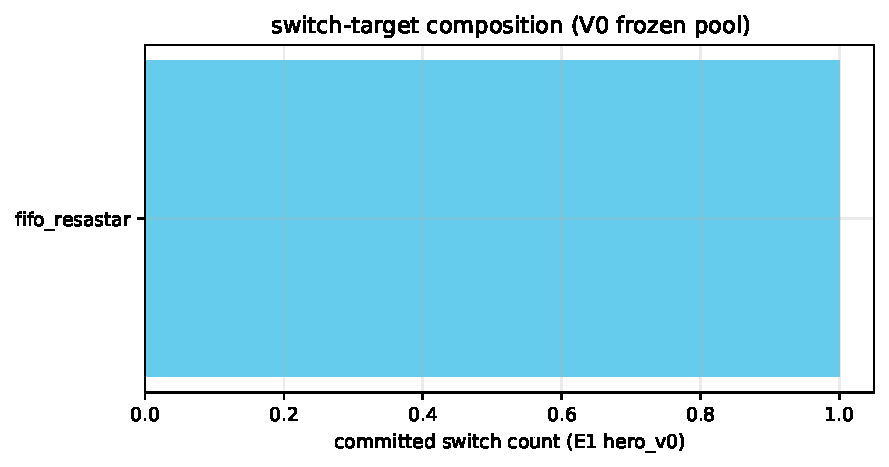
\includegraphics[width=0.6\textwidth]{figures/v5/fig16_switch_composition.pdf}
\caption{\development V0b 切换目标构成（V0 冻结 12 配方池）。}
\label{fig:v5-switching}
\end{figure*}

\begin{figure*}[t]
\centering
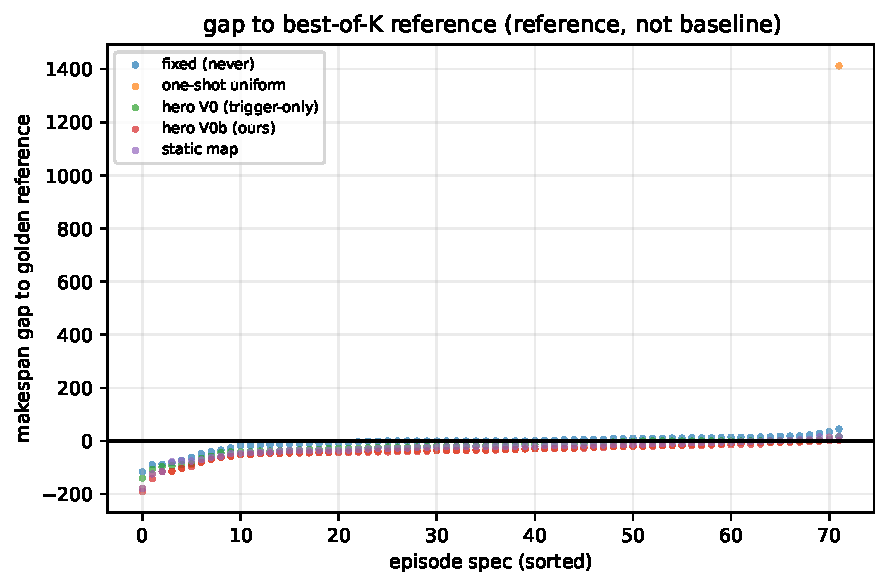
\includegraphics[width=0.8\textwidth]{figures/v5/fig14_golden_gap.pdf}
\caption{\development 各方法相对 golden 参考值的逐 spec 差距
（参考值非基线）。}
\label{fig:v5-gap}
\end{figure*}

\begin{table}[t]
\centering
\caption{\development golden trace round-1 摘要（表 T3；参考值口径，
K 内最优非全局最优，详见协议）。}
\label{tab:golden}
% auto-generated from golden_trace_r1 manifest; do not edit by hand
\begin{tabular}{lrrrrr}
\toprule
workload & specs & golden mean & $K$-median & golden switches & terminal \\
\midrule
burst\_priority & 12 & 143.6 & 244.7 & 2.2 & 84/96 \\
deep\_chain & 12 & 136.4 & 246.2 & 2.8 & 82/96 \\
medium\_balanced & 12 & 126.5 & 184.4 & 1.8 & 96/96 \\
small\_sparse & 12 & 54.3 & 63.6 & 1.8 & 96/96 \\
staggered\_flow & 12 & 134.2 & 214.1 & 2.6 & 87/96 \\
transport\_intensive & 12 & 226.2 & 334.6 & 5.8 & 59/96 \\
\midrule
all & 72 & 136.9 & 132 & 2.8 & 504/576 \\
\bottomrule
\end{tabular}

\end{table}

\section{讨论与边界}
\label{sec:discussion}

\textbf{定位边界}。本文回答 RQ1--RQ3：反事实模拟基础设施（确认）、真值获取
方法（演示级）、在线深搜索的证伪（paper-grade）。它\emph{不}声称：(i) 隐藏
分数模型可预测 $G$——历史特征混叠诊断（根级 Spearman 0.0048）表明这依赖
尚未完成的表征修复与决策点数据；(ii) \racing{} 已在产业规模场面验证——
演示场面仅验证机制与可复现性。

\textbf{已知威胁}。其一，历史开发根的元数据存在源契约缺陷（配置交期/优先级
未传播至运行时），相关诊断标记为污染特征下的结论；契约已修复并以 fail-loud
校验固化，干净根重采后方可复检。其二，截断统计语义（删失下界 vs 真值）在
正式协议中必须显式定义，否则 ground truth 会被罚值污染。其三，仿真保真度
是全部结论的前提，正式 oracle 运行前需通过"同动作同 Tape 重放原轨迹"的
保真度前置门。

\textbf{后续工作}。按既定路线：golden trace round-1 采集与参考值落盘；
组合空间契约（组合文法/合法性掩码/切换成本表）与 $C_\text{switch}$ 计价
接入；决策点限时组合搜索 V0/V1 实现与强制基线（一次浅搜、uniform）对比
（\ref{sec:target} 节，RQ4）；$LCB(G)>\tau$ 切换层 shadow 激活；随机轨迹
自然实验的切换因果分析；闭环双口径评估收尾。逐决策点 oracle 标签重算与
预测器训练、采样分布的 expert iteration（round$\geq$2）、对象级调度解搜索
与 LLM 联合调度作为独立后续方向另行报告，本文架构即其 baseline 与打分
来源。

\textbf{目标架构的特有风险}。其一，元级搜索重演深控陷阱：四条硬约束
（\ref{sec:target} 节）是唯一防线，及格线为一次浅搜与 uniform，不合格即
如实报告。其二，真值语义漂移：best-of-$K$ 参考值、冻结集穷举值与在线估计
三种口径并存，任何场合混用即构成过度声明。其三，因果分析边界：配对克隆
层的结论上限为仿真保真度，且被 CP-SAT 非确定性限制（排除或增补 Tape）；
自然实验结论只覆盖随机策略可达的状态—动作分布；事件研究带选择偏差——
三层报告范围不得互换。其四，V0/V1 口径分离：开放组合空间的收益必须与
"自适应本身"的收益分离报告。其五，baseline 公平性：LLM 对比实验中禁止
给任一方更宽松的预算或动作空间。

\section{结论}
\label{sec:conclusion}

本文把闭环 FJSP--MAPF 中的求解与评估重组为一个统一问题：在连续物理时钟下
对候选动作做反事实模拟，并以同一个 anytime 搜索回答两个方向的问题——限定
时间时在组合空间给出切换决策，解除限制并冻结集合时给出精确验证值。我们
交付了经独立确认的反事实基础设施；以 936 个配对 episode 透明证伪了元级
\emph{周期性深度控制}，并把它与被证据支持的决策点浅搜形态划清边界；实现了
具备穷举退化性质与 anytime 保证的 \racing{} 竞赛评估器；给出决策点限时
组合搜索与成本感知切换的完整目标架构——两级候选构造、golden trace 参考
真值、配对克隆反事实与随机自然实验互证的因果分析（含估计量显式定义与
离策略评估接口）、以及双口径评估协议。核心立场是：算子组合
不由人定，由预算受限的搜索在线产生；切换必须显式计价、由置信下界拍板；
真值必须分层声明；质量与开销分开记账；比较必须同源同预算。

\bibliographystyle{plainnat}
\bibliography{references_counterfactual_v4}

\end{document}
